% !TEX root = ../main.tex

\section{Ветер2} 
\textbf{Геострофический ветер} - градиентный ветер при прямолинейных изобарах.\\
\textbf{Геоциклострофический ветер} - градиентный ветер при криволинейных изобарах.\\

\begin{wrapfigure}[8]{R}{0.51\linewidth}
	\vspace{-5ex}
	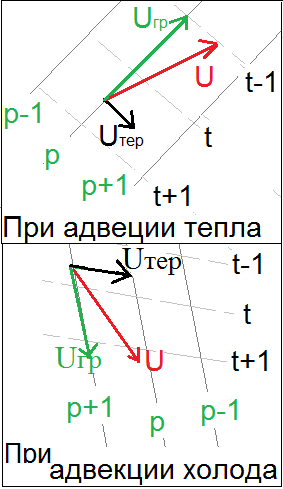
\includegraphics[width=28 mm]{Thermal_wind}
\end{wrapfigure}

\textbf{Термический ветер} - прирост геострофического ветра от одного уровня к др за счет ср гориз-ого градиента T в слое между этими уровнями.\\
Тёплый воздух, стараясь выровнять T, устремляется в сторону более холодного; поток воздуха устойчив тогда, когда будет направлен параллельно изотермам (область холодного слева в С полушарии).\\
При адвекция тепла наблюдается правый поворот ветра (по ч.c), а при адвекция холода - левый поворот.

\par\textbf{Эквивалентный ветер} (вспоминай навигу) позволяет определить фактическую W при известной V и требуемую V для полета по расписанию c заданной W.\\

\underline{\textbf{Воз/ потоки в основных бар-их системах:}}
В циклоне $F_{\text{гр}}$ и ветер направлены к центру, в антициклоне - к периферии.

\begin{wrapfigure}[7]{R}{0.51\linewidth}
	\vspace{-8ex}
	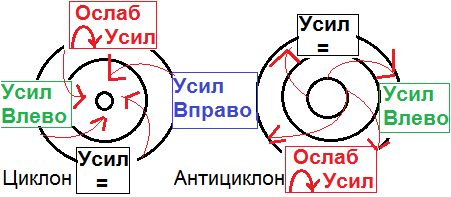
\includegraphics[width=28 mm]{Cyclon}
\end{wrapfigure}

В передней части циклона и на западной периферия антициклона ветер \textcolor{blue}{усиливается и поворачивает в право} \\
В тылу циклона и на восточной периферии антициклона \textcolor{Green}{усиливается и поворачивает влево}\\
В южной части циклона и в северной части антициклона \textbf{усиливается не меняя направление}\\
В северной части циклона и в южной части антициклона \textcolor{red}{ослабевает} На некотором уровне меняет свое направление на противоположное после чего усиливается.
 
\par При изменении ветра с H его напр приближается к направлению к $\parallel$ изотермам.\\
\textbf{Ведущий поток} - ветровой поток однородного напр-ия, который образуется на некоторой высоте (обычно 3-5 км). По нему перемещаются циклоны и антициклоны, приземные центры которых распол-ся под этим потоком. Скорость перемещения бар. систем составляет 80\% от $V_{cp}$ ведущего потока на 3 км или 50\% на 5 км.
\par \textbf{Центр циклона} на высоте смещен относительно произвольного центра в область холода, а \textbf{центр антициклона} - в область тепла.
\par Правое вращение ветра с высотой в свободной атмосфере является признаком наступающего потепления и приближения передней части циклона. Левое вращение характеризует вторжение холодного воздуха и приближение передней части антициклона.

\par \underline{\textbf{Ветер и его влияние на полёт}}\\
Хар-ки приземного ветра влияют на взлет/посадку\\
ветер на высотах - на нав. элементы полета.\\
При сильном ветре на а/д могут возникать: метели и пыльные бури, которые ухудшают гор. видимость ниже минимума погоды а/д.\\
Ураганы и шквалы при взлете/посадке могут приводить к летным происшествием.\\
Турбулентность атмосферы вызывает интенсивную болтанку и броски ВС.\\
Для обеспечения безопасности полетов и выполнения их по расписанию ветер учитывается при всех нав расчетах.\\
Климатические хар-ки ветра учитываются при строительстве а/м и составлении расписания движения на воз трассах.\\ 
При выполнении гор полета ветер влиянет на W и УС при V=, от напр-я и U ветра зависит продолжительность полета по воз трассе, при боковом ветре ПУ будет отличаться от КУ.\\
Ветер влияет на взлетно посадочные хар-ки: длину разбега, V отрыва, длину пробега и посадочную V. Наиболее благоприятным для взлета и посадки является встречный ветер, т.к. все перечисленные взлетно-посадочные хар-ки имеют меньшую величину и самолет имеет лучшую устойчивость и управляемость.